\documentclass[superscriptaddress,floatfix,draft,prl]{revtex4-1}
\usepackage{epsfig,hyperref,graphics,float,amsmath,mathtools}
\usepackage{microtype,setspace,siunitx,physics,epsfig,graphicx}
\usepackage[caption=false]{subfig}
\usepackage{xcolor}
\usepackage{nameref}
\captionsetup[subfigure]{labelformat=brace}

\begin{document}
\bibliographystyle{apsrev4-1}


\title{The XY Model in Freely-Suspended Nanofilms of Liquid Crystal}
\date{\today}

\author{Adam A.~S.~Green}
\affiliation{Department of Physics and Soft Materials Research Center,
University of Colorado Boulder, Boulder, CO, 80309-0390, USA}

\author{Stian M. Howard}
\affiliation{Department of Physics and Soft Materials Research Center,
University of Colorado Boulder, Boulder, CO, 80309-0390, USA}

\author{Eric A. Minor}
\affiliation{Department of Physics and Soft Materials Research Center,
University of Colorado Boulder, Boulder, CO, 80309-0390, USA}



\author{Cheol S.~Park}
\affiliation{Department of Physics and Soft Materials Research Center,
University of Colorado Boulder, Boulder, CO, 80309-0390, USA}

\author{Noel A.~Clark}
\affiliation{Department of Physics and Soft Materials Research Center,
University of Colorado Boulder, Boulder, CO, 80309-0390, USA}


\newcommand{\jem}[1]{{{\color{black} #1}}}

\begin{abstract}

\end{abstract}



\maketitle

\section{Introduction}
1. An introduction to freely suspended films
1. a) defect structure
2. An introduction to the XY model (energy scaling of defects, Yurke, dynamic scaling
proof, open question of whether or not the XY model is applicable to freely
suspended films
3. Both 1 and 2



\section{Experimental Design}
1. Modify the picture so it isn't exactly the same figure maybe?
2. Discuss the picture and setup and how the quenching is produced
3. Show image frame with machine learning, discuss the machine learning method used to detect the
defects

A sealed, cylindrical chamber with a
\SI{5}{\milli\metre} aperture hole ultra-sonically drilled into the top glass
plate was constructed to allow a freely-suspended film to be mechanically
quenched. 
\begin{figure}[h!]
    \centering
    
\includegraphics[width=.6\textwidth]{/mnt/c/Users/rings/Documents/Work/thesis/written/main/figs/topo/quench-chamber.png}
    \caption[Schematic of quench chamber]{\label{fig:topo:quenchChamber}Pressure
        quench chamber. A
        \SI{1.82}{\centi\meter} outer diameter aluminum cylinder
        \SI{4.43}{\centi\meter} tall was drilled through to give a \SI{10.00}{\milli\meter} hole. A glass cover slip was affixed with vacuum epoxy at a
Brewster's angle of \SI{57}{\degree} to seal the bottom. A glass coverslip with
a \SI{5.00}{\milli\meter} hole ultrasonically drilled through was affixed with
vacuum epoxy on the top of the chamber. The freely-suspended film drawn
across this aperture creates a liquid airlock that allows the chamber to be
pressurized.}
\end{figure}
Air is injected into the system by means of a syringe coupled to a
micrometer, which, when a freely-suspended film is sealing the top aperture,
causes the film to bulge upwards, forming a dome.

\begin{figure}[h!]
    \centering
    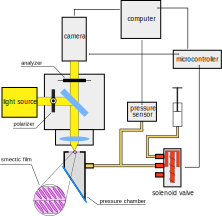
\includegraphics[width=.8\textwidth]{/mnt/c/Users/rings/Documents/Work/thesis/written/main/figs/topo/quench-schematic.png}
    \caption[Schematic of quench
    experiment.]{\label{fig:topo:quenchSchematic}Schematic of quench experiment.
    The syringe is coupled to a translation stage, allowing for fine control.
When depressed, the compression increases the pressure in the quench chamber,
causing the film to bulge outwards. The pressure is monitored by a pressure
sensor (Honeywell SDX010IND4) which outputs a proportional voltage read by a
digital multimeter connected serially to a computer. The user can enter a
target threshold pressure in a program running on the computer, which
automatically triggers a quench when said threshold is reached. The quench is
triggered by sending a digital signal to a connected microcontrolled (Arduino
Uno) which first instructs the high-speed (Phantom V12.2) camera to begin
recording and then opens the solenoid valve, venting the system to atmosphere.
The resulting dynamics on the film are captured by the camera as a video, which
is then transferred to the computer for further analysis.}
\end{figure}




As the deformed film is incompressible to first order, it must pull in material from the meniscus to account for the
increase in surface area. When the appropriate pressure is reached, a solenoid
pressure value is electronically triggered, which instantly opens the chamber to the
atmosphere. The resulting rapid decrease in pressure collapses the dome. If the
dome collapses faster than material can be transported back to the meniscus,
there is a temporary increase in density and in-plane pressure, which forces the film to transition to
an untilted, SmA state. Once the dome has collapsed completely, the in-plane
pressure returns to its equilibrium value and the system rapidly re-enters the
SmC phase. Practically, this has the same effect as a rapid temperature quench,
where the system is adiabatically taken from a SmA phase to a SmC phase, which makes it a useful system to compare to
the computer simulations by Yurke and subsequent models. 

The return to an equilibrium configuration from an initial quench takes between
a
second and a minute, depending on the temperature and specific quench conditions,
requiring the use of high-speed video microscopy to capture these dynamics.
\autoref{fig:topo:qm} shows a montage of images taken from a typical
high-speed video, where the evolution of the system can be clearly tracked.
\begin{figure}[h!]
    \centering
    \includegraphics[width=.8\textwidth]{/mnt/c/Users/rings/Documents/Work/thesis/written/main/figs/intro/quenchMontage/qM.png}
    \caption[Montage of still frames from mechanically quenched film (material
    PM2) viewed
    under reflection.]{\label{fig:topo:qm}Annihilation of defects after a quench. This
        series of images are frames taken from a high-speed video which recorded
        the quench dynamics as the system approaches equilibrium. The defects at
        located at the `knot' of each bowtie, as the four brushes of the
        four-fold degenerate Schlieren texture become two under decrossed polarizers. The pre-quench
        pressure was \SI{57}{\pascal} with the temperature of the chamber held
    at \SI{30}{\degreeCelsius}.}
    \end{figure}

The first version, which allowed micrometer control
over the XY stage, had insufficient chamber depth, causing optical
artifacts from back reflections. The improved, and currently used setup,
was redesigned to give maximum separation from the bottom of the chamber to the focal-plane where the film is
viewed. A pressure sensor (Honeywell SDX010IND4) was also
integrated into the system, which, when combined with a low-noise high-gain
instrumentational amplifier reading onto a microcontroller
(Arduino Uno) allows for high-resolution measurement of the
pressure during a quench. The pressure sensor measures a differential pressure,
so in principle, only the pressure immediately preceding a quench needs to be
recorded ($p(t_0)$). However, it was found that the offset voltage of the
pressure sensor was temperature sensitive, and could vary significantly in time.
\begin{figure}[h!]
    \centering
    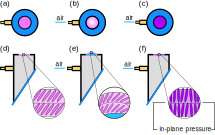
\includegraphics[width=.9\textwidth]{/mnt/c/Users/rings/Documents/Work/thesis/written/main/figs/topo/quench-sequence.png}
    \caption[Outline of mechanical quench
    sequence.]{\label{fig:topo:quenchSequence}Outline of mechanical quench
        sequence in both top (a-c) and bottom (d-f) view. (a,d) The SmC film is
        in an equilibrium position. (b,d) as the chamber is
    pressurized, the film bulges outward. (c,f) When the chamber is quenched,
the film collapses back to a flat configuration, temporarily increasing the
in-plane pressure.}
\end{figure}

This meant that the pressure measuring setup was overly susceptible to slow temperature
fluctuations, which caused a slow drift in the pressure sensor's offset voltage
which was amplified by the subsequent electronics.
This means that the equilibrium pressure needed to be monitored ($p(t_f)$). The
This makes the data precise but
not accurate. As the dynamics of the system can change dramatically with
relatively small variations in the pressure, a new approach was taken. Instead
of amplifying the signal, we used a high-resolution digital multimeter
interfaced directly to the computer. Though the multimeter was
unable to achieve the high time resolution of the microcontroller, it was
significantly more accurate, allowing quenching experiments to be run repeatably
under the same conditions. Another benefit was that the digital multimeter was
not limited by onboard memory considerations, as the data was streamed directly
to the computer, allowing for arbitrary durations of the experiment. Though unable to
resolve the dynamics of the quench, we gained better accuracy for our measurements
of $\Delta p=p(t_f)-p(t_0)$.

\begin{figure}[h!]
    \centering
    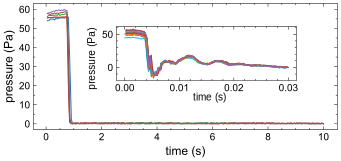
\includegraphics[width=.8\textwidth]{/mnt/c/Users/rings/Documents/Work/thesis/written/main/figs/topo/pressure/topo-pressures.png}
    \caption[Pressure of quench chamber during mechanical quench event.]{\label{fig:topo:quenchPressures} Pressure during the quench for the
        data sets used in this thesis as monitored directly (unamplified) by a
        digital multimeter connected to a computer. They are all well clustered between
    \SIrange{55}{60}{\pascal}. The inset shows the high-resolution time data
afforded by the previous setup, where an amplified signal was read into a
microcontroller.}
\end{figure}


The range of pressures over which a useful quench could be gathered was limited,
as it was found that increasing the pressure over a threshold ($p_\textrm{th} >
\SI{65}{\pascal}$)
meant that the resultant increase of the energy of the film overcame the
island-nucleation barrier, and the isotropic conditions necessary to compare the
quenched textures to theory were broken by the nucleated islands. It is worth
noting that, though this island nucleation is not the focus of this chapter, it
is an active area of investigation for the Boulder group, with an interest in
studying island-mediated nucleation of long-lived defect structures. 


%discuss difficulty in achieving pressure data/isolation (calculate average
%pressure flucuation at standard conditions)
%show high-resolution pressure data, (interesting, don't understand it though)
%show low-resolution pressure data

Though several materials were tried, the best material was found to be
\textbf{PM2}: a 50:50 mixture by weight between SYNTHON ST00552
(2-(4-n-Hexyloxyphenyl)-5-n-octylpyrimidine) and SYNTHON ST00557
(5-n-Decyl-2-(4-n-octyloxyphenyl)pyrimidine), which has a phase sequence of SmC
\SI{52}{\degreeCelsius} SmA \SI{68}{\degreeCelsius} N \SI{72}{\degreeCelsius} I. The
chemical structures of these materials is shown in
\autoref{fig:topo:german}\cite{HarthEpisodeslifedeath2016}.

\begin{figure}[h!]
    \centering
    
\includegraphics[width=.6\textwidth]{/mnt/c/Users/rings/Documents/Work/thesis/written/main/figs/topo/compounds/compounds.png}
    \caption[Material used in quench experiments.]{\label{fig:topo:german}
        Mixture \textbf{PM2}, a 50:50 by weight mixture of
        SYNTHON ST00552 and SYNTHON ST00557. ST00557 is
        5-n-Decyl-2-(4-n-octyloxyphenyl)pyrimidine, and ST00552 is
    2-(4-n-Hexyloxyphenyl)-5-n-octylpyrimidine. This gives a room temperature
SmC. All experiments were conducted at \SI{35}{\degreeCelsius}.}
\end{figure}


\section{Results}
1. Show montage image, then show big graph with logarythmic fits, show the Yurke
corrections
2. Show the simulated textures as well, as a confirmation of the results
\section{Conclusion}
We can crib this from our thesis.
%\begin{figure*}
%    \includegraphics[width=2\columnwidth]{Figure1.png}
%    \caption{\label{fig:main} 
%    }
%       \end{figure*}
%
This work was supported by the Soft Materials Research Center under NSF MRSEC
Grant~DMR-1420736 and NSF MRSEC Grant~DMR-1710711, by NASA Grant~NNX-13AQ81G, and by DFG Grant~Ts~39/24-2.
RSoXS measurements were made at the Advanced Light Source, which is a DOE Office of Science User Facility operated under Contract No.~DE-AC02-05CH11231. We acknowledge the assistance of beamline scientist Cheng Wang.
SAXS measurements were carried out at the National Synchrotron Light Source, a U.S. Department of Energy (DOE) Office of Science User Facility operated for the DOE Office of Science by Brookhaven National Laboratory under Contract No.~DE-AC02-98CH10886.

Further experimental details and additional figures are provided in the Supplemental Materials \cite{supplement}.
\bibliography{topo}
\end{document}

